\documentclass[dvisvgm,tikz,border=8pt]{standalone}
\usepackage{amsmath,amssymb}
\usetikzlibrary{arrows}
\begin{document}
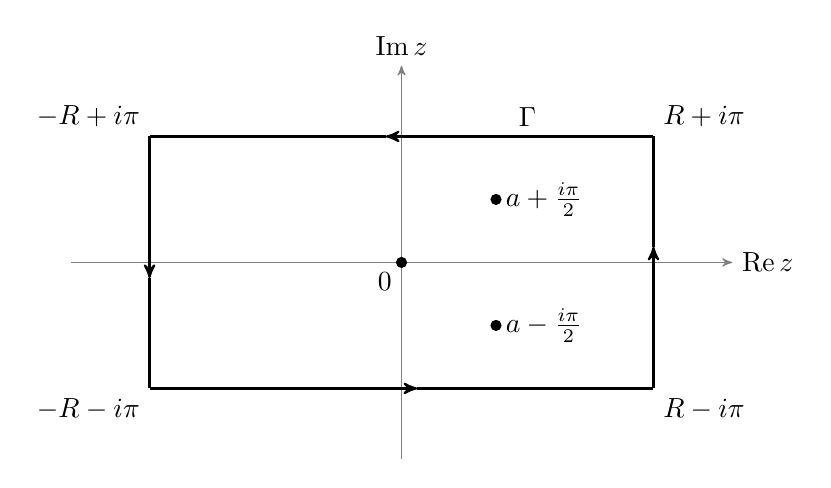
\begin{tikzpicture}
\draw[->,>=stealth',gray] (-4.2,0) -- (4.2,0) node[right,black] {$\operatorname{Re} z$};
\draw[->,>=stealth',gray] (0,-2.5) -- (0,2.5) node[above,black] {$\operatorname{Im} z$};
\draw[thick,->,>=stealth'] (-3.2,-1.6) -- (0.2,-1.6);
\draw[thick] (0.2,-1.6) -- (3.2,-1.6);
\draw[thick,->,>=stealth'] (3.2,-1.6) -- (3.2,0.2);
\draw[thick] (3.2,0.2) -- (3.2,1.6);
\draw[thick,->,>=stealth'] (3.2,1.6) -- (-0.2,1.6);
\draw[thick] (-0.2,1.6) -- (-3.2,1.6);
\draw[thick,->,>=stealth'] (-3.2,1.6) -- (-3.2,-0.2);
\draw[thick] (-3.2,-0.2) -- (-3.2,-1.6);
\filldraw[black] (0,0) circle[radius=1.8pt] node[below left] {$0$}
                 (1.2,0.8) circle[radius=1.8pt] node[right] {$a+\frac{i\pi}{2}$}
                 (1.2,-0.8) circle[radius=1.8pt] node[right] {$a-\frac{i\pi}{2}$};
\draw (3.2,-1.6) node[below right] {$R-i\pi$}
      (3.2,1.6) node[above right] {$R+i\pi$}
      (-3.2,1.6) node[above left] {$-R+i\pi$}
      (-3.2,-1.6) node[below left] {$-R-i\pi$}
      (1.6,1.6) node[above] {$\Gamma$};
\end{tikzpicture}
\end{document}

